\documentclass[journal]{IEEEtran}

%% Packages
\usepackage{cite}
\ifCLASSINFOpdf
  \usepackage[pdftex]{graphicx}
  \graphicspath{{../pdf/}{../jpeg/}}
  \DeclareGraphicsExtensions{.pdf,.jpeg,.png}
\else
  \usepackage[dvips]{graphicx}
  \graphicspath{{../eps/}}
  \DeclareGraphicsExtensions{.eps}
\fi
\usepackage[cmex10]{amsmath}
%\usepackage{algorithm}
\usepackage{algorithmic}
\usepackage{array}
\usepackage{mdwmath}
\usepackage{mdwtab}
\usepackage{eqparbox}
\usepackage[caption=false,font=footnotesize]{subfig}
\usepackage{fixltx2e}
%\usepackage{stfloats}
\usepackage{url}

% correct bad hyphenation here
\hyphenation{op-tical net-works semi-conduc-tor}


\begin{document}

\title{Improved Particle Approximations \\ to the Joint Smoothing Distribution \\ Using Markov Chain Monte Carlo}

\author{Pete~Bunch,~\IEEEmembership{}
        Simon~Godsill,~\IEEEmembership{Member,~IEEE,}% <-this % stops a space
\thanks{P. Bunch and S. Godsill are with the Department
of Engineering, Cambridge University, UK. email: \{pb404,sjg30\}@cam.ac.uk}% <-this % stops a space
\thanks{Manuscript received January 01, 1901; revised January 02, 1901.}}

% The paper headers
\markboth{IEEE Transaction in Signal Processing,~Vol.~1, No.~1, January~1901}%
{Bunch \& Godsill \MakeLowercase{\textit{et al.}}: Improved Particle Approximations to the Joint Smoothing Distribution Using Markov Chain Monte Carlo}

% make the title area
\maketitle


\begin{abstract}
Particle filtering and smoothing algorithms approximate posterior state distributions with a set of samples drawn from those distributions. Conventionally, samples from the joint smoothing distribution are generated by sequentially resampling from the particle filter results. If the number of filtering particles is high, this process is limited by computational complexity. In addition, the support of the smoothing distribution is restricted to the values which appear in the filtering approximation. In this paper, a Markov chain Monte Carlo sampling procedure is used to improve the efficiency of the particle smoother. In addition, an algorithm for approximating the joint smoothing distribution without limited support is presented.
\end{abstract}



\begin{IEEEkeywords}
state space model, particle filter, smoothing, MCMC, Bayesian inference
\end{IEEEkeywords}



\section{Introduction} \label{sec:intro}

\IEEEPARstart{T}{he} objective of sequential Bayesian inference is the estimation of an unknown, time-varying quanitity from incomplete or inaccurate observations. This is commonly achieved through the use of discrete-time probabilistic models for the evolution of the latent state and the measurement process, defined by transition and observation densities.

\begin{IEEEeqnarray}{rCl}
x_{k} & \sim & p(x_{k}|x_{k-1}) \label{eq:state_proc}\\
y_{k} & \sim & p(y_{k}|x_{k})   \label{eq:observ_proc}
\end{IEEEeqnarray}

Here, the random variable $x_k$ denotes the value of the latent state at the $k$th instant, and $y_k$ the value of the observation. A set of random variables will be written as $x_{1:k} = \{x_1, x_2, \dots, x_k \}$. The state evolution is assumed to be Markovian, i.e. $x_k$ depends only on the previous value, $x_{k-1}$.

Commonly of interest are the problems of filtering and smoothing. Filtering is the inference of $p(x_k|y_{1:k})$, the distribution of the current state given all previous observations. Smoothing consists of two related tasks, the inference of $p(x_{1:K}|y_{1:K})$ (where $K$ is the number of time steps), the joint distribution of the entire state sequence given all the observations, and that of $p(x_{k}|y_{1:K})$, the marginal distribution of each state given all the observations. In this paper, we are concerned with the estimation of the joint smoothing distribution.

In the case where the state and observation processes of (\ref{eq:state_proc}) and~(\ref{eq:observ_proc}) are linear and Gaussian, the filtering problem may be solved analytically using the Kalman filter \cite{Kalman1960}. For nonlinear or non-Gaussian models, tractable closed-form solutions are rare. Instead, numerical approximations are often employed, including the particle filter algorithm, first introduced by \cite{Gordon1993}. (See \cite{Cappe2007,Doucet2009} for a thorough introduction.)

In a particle filter, the filtering distribution is approximated by a set of weighted samples (or ``particles'') drawn from that distribution.

\begin{IEEEeqnarray}{rCl}
\hat{p}(x_{k}|y_{1:k}) & = & \sum_i w_k^{(i)} \delta_{x_k^{(i)}}(x_k)
\end{IEEEeqnarray}

Here, $\delta_{a}(x)$ indicates a discrete probability mass at the point $x = a$.% $\hat{p}$ means an approximation to $p$.

A similar story applies to the problem of smoothing. In the linear Gaussian case, the entire state sequence, $x_{1:K}$, may be estimated in closed-form using the a Rauch-Tung-Striebel (RTS) smoother \cite{Rauch1965}. This works by modifying the ordinary Kalman filter results in a backward processing pass through the state sequence. For nonlinear or non-Gaussian models, it is possible again to resort to numerical methods. Now, particles are used to approximate the joint smoothing distribution.

\begin{IEEEeqnarray}{rCl}
\hat{p}(x_{1:K}|y_{1:K}) & = & \sum_i w_K^{(i)} \delta_{x_{1:K}^{(i)}}(x_{1:K})
\end{IEEEeqnarray}

Each particle is an entire realisation of the state process, with $K$ values corresponding to the state at each time step. Methods for generating these samples have been described in \cite{Kitagawa1996,Godsill2004,Briers2010}. In this paper new algorithms are presented for drawing samples from the joint smoothing distribution, using Markov chain Monte Carlo (MCMC). These novel procedures have computational advantages and greater flexibility over previous methods.

In section~\ref{sec:basics}, we briefly review the basic particle filter and existing joint smoother algorithms. The new MCMC-based smoothing methods are presented in sections~\ref{sec:mcmc_smoother} and~\ref{sec:new_state_smoother} with supporting simulations in section~\ref{sec:simulations}.



\section{Particle Filtering and Smoothing} \label{sec:basics}

\subsection{The Particle Filter}

The particle filter is a recursive numerical algorithm for estimation of the filtering distribution. At the $k$th processing step, a particle estimate of the joint density over $x_{k-1}$ and $x_k$ is made using importance sampling (IS). A particle is first sampled from the factorised proposal density,

\begin{IEEEeqnarray}{rCl}
\{ x_{k-1}^{(i)}, x_k^{(i)} \} & \sim & q(x_{x}|x_{k-1}) q(x_{k-1}).
\end{IEEEeqnarray}

The proposal density for $x_k$, $q(x_{x}|x_{k-1})$, is often called the ``importance density''. Common choices include the model transition density (\ref{eq:state_proc}), and the ``optimal importance distribution'' \cite{Doucet2000a}. The proposal density for $x_{k-1}$, $q(x_{k-1})$, is constructed from the particles of the filtering approximation from the previous time step. The choice of weights and sampling procedure for $x_{k-1}$ determines what from of ``resampling'' is to be used. Here we use arbitrary weights for generality.

\begin{IEEEeqnarray}{rCl}
q(x_{k-1}) & = & \sum_i v_{k-1}^{(i)} \delta_{x_{k-1}^{(i)}}(x_{k-1})
\end{IEEEeqnarray}

the choice $v_{k-1}^{(i)} = w_{k-1}^{(i)}$ corresponds to ordinary resampling, and other choices of $v_{k-1}^{(i)}$ represent auxiliary sampling schemes \cite{Pitt1999}. For the least computational expense, the proposal density with weights $v_{k-1}^{(i)} = 1/N_F$ (where $N_F$ is the number of filter particles) can be ``sampled'' by simply keeping the set of particles generated in the last step, with no resampling. (See \cite{Douc2005} for further discussion of resampling.)

Next, the particles are assigned an importance weight according to the ratio of the target and the proposal densities.

\begin{IEEEeqnarray}{rCl}
w_{k}^{(i)} & =       & \frac{ p(x_{k-1}^{(i)}, x_k^{(i)}|y_{1:k}) }{ q(x_{x}^{(i)}|x_{k-1}^{(i)}) q(x_{k-1}^{(i)}) } \nonumber \\
            & \propto & \frac{ p(y_k|x_k^{(i)}) p(x_k^{(i)}|x_{k-1}^{(i)}) p(x_{k-1}^{(i)}|y_{1:k-1}) }{ q(x_{x}^{(i)}|x_{k-1}^{(i)}) q(x_{k-1}^{(i)}) } \nonumber \\
            & \approx & \frac{ p(y_k|x_k^{(i)}) p(x_k^{(i)}|x_{k-1}^{(i)}) }{ q(x_{x}^{(i)}|x_{k-1}^{(i)}) } \times \frac{w_{k-1}^{(i)}}{v_{k-1}^{(i)} }
\end{IEEEeqnarray}

Normalisation is enforced by scaling the weights so that they sum to 0. Finally, $x_{k-1}$ is marginalised from the distribution by simply discarding the values from each particle.

The particle filter is summarised in Fig.~\ref{alg:PF}.

%\begin{algorithm}
\begin{figure}
\fbox{\parbox{\columnwidth}{
\begin{algorithmic}[1]
	\STATE Initialise particles from prior, $x_{0}^{(i)} \sim p(x_{0})$.
	\FOR{$k = 1$ \TO $K$}
 		\FOR{$i = 1$ \TO $N_F$}
 			\STATE Sample $\{ x_{k-1}^{(i)}, x_k^{(i)} \} \sim \sum_j v_{k-1}^{(j)} q(x_k|x_{k-1}^{(j)})$.
 			\STATE Weight $w_{k}^{(i)} \propto \frac{ p(y_k|x_k^{(i)}) p(x_k^{(i)}|x_{k-1}^{(i)}) }{ q(x_{x}^{(i)}|x_{k-1}^{(i)}) } \times \frac{w_{k-1}^{(i)}}{v_{k-1}^{(i)} }$.
 			\STATE Discard $x_{k-1}^{(i)}$.
 		\ENDFOR
 	  \STATE Scale weights so that $\sum_i w_{k}^{(i)} = 1$.
 	\ENDFOR
\end{algorithmic}
}}
\caption{Particle filter algorithm}
\label{alg:PF}
\end{figure}
%\end{algorithm}

\subsection{Existing Algorithms for Particle Smoothing }

The particle filter generates a numerical approximation to each filtering distribution, $p(x_k|y_{1:k})$ by simulating a set of samples from each. A similar sampling-based method may be used to estimate the smoothing distribution.

The most basic particle smoother was presented in \cite{Kitagawa1996}, and is a trivial extension of the particle filter. Rather than marginalising the previous states from each particle, these past values are stored as well. Thus, at each step the algorithm generates an approximation to $p(x_{1:k}|y_{1:k})$. The output from the final processing step is an approximation to the desired smoothing distribution.

The weakness of this simple, filter-smoother (FS) is degeneracy of the particles in the path-space. Every time the particles are resampled, those with low weights do not appear in the approximation at the next step, while those with high weights appear multiple times. The result is that many, or even all, particles will share a common ancestor, before which they all have the same set of state values. If the objective is only to produce a single point estimate then this might be sufficient, but to characterise the complete smoothing distribution, the path-space diversity of the approximation must be improved.

The filter-smoother is summarised in Fig.~\ref{alg:FS}.

%\begin{algorithm}
\begin{figure}
\fbox{\parbox{\columnwidth}{
\begin{algorithmic}[1]
 	\STATE Initialise particles from prior, $x_{0}^{(i)} \sim p(x_{0})$.
 	\FOR{$k = 1$ \TO $K$}
 		\FOR{$i = 1$ \TO $N_F$}
 			\STATE Sample $\{ x_{1:k-1}^{(i)}, x_k^{(i)} \} \sim \sum_j v_{k-1}^{(j)} q(x_k|x_{k-1}^{(j)})$.
 			\STATE Weight $w_{k}^{(i)} \propto \frac{ p(y_k|x_k^{(i)}) p(x_k^{(i)}|x_{k-1}^{(i)}) }{ q(x_{x}^{(i)}|x_{k-1}^{(i)}) } \times \frac{w_{k-1}^{(i)}}{v_{k-1}^{(i)} }$.
 		\ENDFOR
 	  \STATE Scale weights so that $\sum_i w_{k}^{(i)} = 1$.
 	\ENDFOR
\end{algorithmic}
}}
\caption{Filter-smoother algorithm}
\label{alg:FS}
\end{figure}
%\end{algorithm}

An improved particle smoothing algorithm was presented in \cite{Godsill2004}. This works by constructing new particles from the smoothing distribution by resampling from the filtering approximations. The sampling procedure exploits the following factorisation of the joint distribution.

\begin{IEEEeqnarray}{rCl}
p(x_{1:K}|y_{1:K}) & = & p(x_K|y_{1:K}) \prod_{k=1}^{K-1} p(x_k|x_{k+1}, y_{1:K}) \label{eq:smoothing_factorisation}
\end{IEEEeqnarray}

Particles are generated by sampling backwards in time from the factors of this expansion. At the $k$th step, a sample $\tilde{x}_{k+1:K} \sim p(x_{k+1:K}|y_{1:K})$ will already have been drawn. By sampling $x_k \sim p(x_k|\tilde{x}_{k+1}, y_{1:K})$ and appending $x_k$ to $\tilde{x}_{k+1:K}$, the state sequence is sequentially extended back in time. The recursion is initialised with $x_K \sim p(x_K|y_{1:K})$, i.e. a sample from the final filtering approximation.

The backwards conditional density may be expanded with Bayes rule.

\begin{IEEEeqnarray}{rCl}
p(x_k|\tilde{x}_{k+1}, y_{1:K}) & =       & p(x_k|\tilde{x}_{k+1}, y_{1:k}) \nonumber \\
                                & \propto & p(\tilde{x}_{k+1}|x_k) p(x_k|y_{1:k})
\end{IEEEeqnarray}

Substituting the filtering approximation into this expression yields a particle distribution which may be sampled easily.

\begin{IEEEeqnarray}{rCl}
\hat{p}(x_k|\tilde{x}_{k+1}, y_{1:K}) = \sum_i  \tilde{w}_k^{(i)} \delta_{x_{k}^{(i)}}(x_{k}) \label{eq:backward_conditional_filter} \\
\tilde{w}_k^{(i)} \propto w_k^{(i)} p(\tilde{x}_{k+1}|x_k^{(i)}) \label{eq:DBRS_weights}
\end{IEEEeqnarray}

The procedure may be repeated to produce as many samples from the joint smoothing distribution as required. This backward-resampling smoother is summarised in Fig.~\ref{alg:DBRS}.

%\begin{algorithm}
\begin{figure}
\fbox{\parbox{\columnwidth}{
\begin{algorithmic}[1]
 	\STATE Run a particle filter to approximate $p(x_k|y_{1:k})$ for each $k$.
	\FOR{$i = 1$ \TO $N_S$}
		\STATE Sample $\tilde{x}_{K}^{(i)} \sim \sum_j w_K^{(j)} \delta_{x_{K}^{(j)}}(x_{K})$.
		\FOR{$k = K-1$ \TO $1$}
			\FOR{$j = 1$ \TO $N_F$}
				\STATE Calculate weight $\tilde{w}_k^{(j)} = w_k^{(j)} p(\tilde{x}_{k+1}|x_k^{(j)})$.
			\ENDFOR
			\STATE Sample $\tilde{x}_{k}^{(i)} \sim \sum_j \tilde{w}_k^{(j)} \delta_{x_{k}^{(j)}}(x_{k})$.
		\ENDFOR
	\ENDFOR
\end{algorithmic}
}}
\caption{Direct backward-resampling smoother algorithm}
\label{alg:DBRS}
\end{figure}
%\end{algorithm}

A method for drawing samples from the joint smoothing distribution, $p(x_{1:K}|y_{1:K})$, is included in \cite{Briers2010}. The principal topic of this paper is a two-filter smoother for estimation of the marginal smoothing distributions, $p(x_{k}|y_{1:K})$, by combination of the results from one forward and one backward particle filter. Particles from the joint distribution may then be generated by resampling from either the forward or backward filters (or some combination) in the manner of the backward-resampling smoother outlined above.%algorithm~\ref{alg:DBRS}.

The complexity of both the backward-resampling smoother of \cite{Godsill2004} and the two-filter variant of \cite{Briers2010} is $\mathcal{O}(N_F \times N_S \times K)$, where $N_F$ is the number of filter particles, $N_S$ the number of smoother particles, and $K$ the number of time steps. Methods for approximation of such algorithms with lower complexity are discussed in \cite{Klaas2006}. However, computational cost is often prohibitive, requiring either $N_S$ or $N_F$ to be held very low. 

In the algorithms described so far, no new states are sampled during the smoothing stage; there is only a resampling of the filtering distributions. This limits the support of the smoother to the states that appear in the filtering particles. In \cite{Fearnhead2010}, an IS-based algorithm for estimation of the marginal smoothing distributions is described in which new states are sampled from a proposal, allowing full support. In addition, this algorithm achieves $\mathcal{O}( N_S \times K)$ complexity, linear in the number of particles.

%In section~\ref{sec:mcmc_smoother}, we introduce an MCMC approach for drawing samples from the joint smoothing distribution with an improved computational complexity over the direct backward-resampling smoother. In section~\ref{sec:new_state_smoother}, we combine this procedure with the new-proposal method used in \cite{Fearnhead2010} to generate joint smoothing distribution particles with full support.



\section{New MCMC Particle Smoother} \label{sec:mcmc_smoother}

The bottleneck of the backward-resampling smoother is the calculation of the sampling weights, specified by (\ref{eq:DBRS_weights}). For each smoother particle and for each time step, a weight must be calculated for each of the $N_F$ filter particles, in order to draw a sample from the conditional distribution $\hat{p}(x_k|\tilde{x}_{k+1}, y_{1:K})$. The innovation here is to use Markov chain Monte Carlo (MCMC) to produce these samples instead of sampling directly.

MCMC algorithms are a class of numerical procedures which use a Markov chain to draw dependent samples from a target probability distribution. A thorough introduction can be found in \cite{Gilks1996}. The basic Metropolis-Hastings (MH) \cite{Hastings1970} sampler uses a series of steps in which a new state is drawn from a proposal distribution and accepted with a probability determined by the ratios of the target and proposal densities.

For the direct backward-resampling smoother, the objective at each time step was to draw a sample from $p(x_{k}|\tilde{x}_{k+1}, y_{1:K})$. To simplify the notation and initialisation of chains, the MCMC version will target $p(x_{1:k}|\tilde{x}_{k+1}, y_{1:K})$. Theoretically this means using the particles of the filter-smoother, $\{x_{1:k}^{(i)}\}$, rather than just the filter, $\{x_k^{(j)}\}$, which would require $\mathcal{O}(K^2)$ memory. However, as discussed later, this is not required in practice.

As before, the algorithm begins by first running a particle filter-smoother and then resampling states backwards through time to produce particles from the joint smoothing distribution, using the factorisation of (\ref{eq:smoothing_factorisation}). At the $k$th time step, a Markov chain is used to sample from $p(x_{1:k}|\tilde{x}_{k+1}, y_{1:K})$. The chain is initialised with the output from the previous processing step. As this is itself a sample from the target distribution, no burn-in period is required.

Following an equivalent derivation to that for (\ref{eq:backward_conditional_filter}), the target distribution may be approximated by a particle distribution.

\begin{IEEEeqnarray}{rCl}
\hat{p}(x_{1:k}|\tilde{x}_{k+1}, y_{1:K}) = \sum_i  \tilde{w}_k^{(i)} \delta_{x_{1:k}^{(i)}}(x_{1:k}) \\
\tilde{w}_k^{(i)} \propto w_k^{(i)} p(\tilde{x}_{k+1}|x_k^{(i)}) \label{eq:MCMC-BRS_weights}
\end{IEEEeqnarray}

A valid proposal may be constructed using the particles of the filter-smoother approximation with any arbitrary weights.

\begin{IEEEeqnarray}{rCl}
q(x_{1:k}|\tilde{x}_{k+1}, y_{1:K}) & = & \sum_j \tilde{v}_k^{(j)} \delta_{x_{1:k}^{(j)}}(x_{1:k})
\end{IEEEeqnarray}

If the current state of the chain is $x_{1:k}^{(m)}$, and a new sample is drawn from the proposal $x_{1:k}^{*} \sim q(x_{1:k}|\tilde{x}_{k+1}, y_{1:K})$, then it should be accepted with the following probability:

\begin{IEEEeqnarray}{rCl}
\alpha &=& \min \Bigg[ 1, \frac{ \hat{p}(x_{1:k}^{*}|\tilde{x}_{k+1}, y_{1:K}) q(x_{1:k}^{(m)}|\tilde{x}_{k+1}, y_{1:K}) }{ \hat{p}(x_{1:k}^{(m)}|\tilde{x}_{k+1}, y_{1:K}) q(x_{1:k}^{*}|\tilde{x}_{k+1}, y_{1:K}) } \Bigg] \nonumber \\
       &=& \min \Bigg[1, \frac{ w_k^{*} \tilde{v}_k^{(m)} }{  w_k^{(m)} \tilde{v}_k^{*} } \times \frac{ p(\tilde{x}_{k+1}|x_k^{*}) }{ p(\tilde{x}_{k+1}|x_k^{(m)}) }  \Bigg]  . \label{eq:MCMC-BRS_ap}
\end{IEEEeqnarray}

Note that $w_k^{*}$ indicates the particle weight of the proposed new state, $x_{1:k}^{*}$.

The final state of each chain is used as a sample from the required conditional distribution.

The complete MCMC backward-resampling smoother is summarised in Fig.~\ref{alg:MCMC-BRS}.

%\begin{algorithm}
\begin{figure}
\fbox{\parbox{\columnwidth}{
\begin{algorithmic}[1]
 	\STATE Run a particle filter to approximate $p(x_{1:k}|y_{1:k})$ for each $k$.
	\FOR{$i = 1$ \TO $N_S$}
		\STATE Sample $\tilde{x}_{1:K}^{(i)} \sim \sum_j w_K^{(j)} \delta_{x_{1:K}^{(j)}}(x_{1:K})$.
		\FOR{$k = K-1$ \TO $1$}
			\STATE $x_{1:k}^{(i)(0)} \gets \tilde{x}_{1:k}^{(i)}$.
			\FOR{$m = 1$ \TO $M$}
				\STATE Propose a new state, $x_{1:k}^{(i)*} \sim \sum_j \tilde{v}_k^{(j)} \delta_{x_{1:k}^{(j)}}(x_{1:k})$.
				\STATE With probability $\alpha$ specified by (\ref{eq:MCMC-BRS_ap}),\\ $x_{1:k}^{(i)(m)} \gets x_{1:k}^{(i)*}$. Otherwise, $x_{1:k}^{(i)(m)} \gets x_{1:k}^{(i)(m-1)}$.
			\ENDFOR
			\STATE $\tilde{x}_{1:k}^{(i)} \gets x_{1:k}^{(i)(M)}$
		\ENDFOR
	\ENDFOR
\end{algorithmic}
}}
\caption{MCMC backward-resampling smoother algorithm}
\label{alg:MCMC-BRS}
\end{figure}
%\end{algorithm}

For a practical implementation, it is not necessary to store the complete particles of the filter-smoother approximations, $\hat{p}(x_{1:k}|y_{1:k})$, which would require memory space which scaled quadratically with $K$. As the smoother progresses backwards in time, the earlier states in the sequence are repeatedly overwritten, and so it is not necessary ever to have known them. Thus, it is only necessary to store the last two states in each filter-smoother particle (i.e. $\{x_{k-1}^{(j)}\}$ and $\{x_{k}^{(j)}\}$).

The computational complexity of the MCMC-based algorithm is $\mathcal{O}(M \times N_S \times K)$, where $M$ is the (mean) number of MH steps used for each time step and smoothing particle. The advantage of the new procedure is that $M$ can often be much smaller than $N_F$ and yet achieve almost equal error performance.

With the direct backward-resampling smoother, the only parameter to be chosen is $N_S$, the number of smoother particles. With the MCMC variant, we also have the freedom to set $M$, the number of MH steps in each Markov chain. This controls a trade-off between speed and accuracy/particle diversity. If the chains are short, and the acceptance probabilities low, then this scheme will simply reproduce particles from the filter-smoother. However, when the weights of the conditional distribution approximation (\ref{eq:MCMC-BRS_weights}) are similar, then an independent sample may be produced with only a very short chain.



\section{An MCMC particle smoother with improved support} \label{sec:new_state_smoother}

Smoothers based on backward-resampling, both the direct sampler of \cite{Godsill2004} and the MCMC version outlined in the previous section, are limited by the fact that states are only selected from those which appear in the filtering approximation. If there is a significant difference between the filtering and smoothing densities, then the the particles are unlikely to be in the right locations to represent the smoothing distribution well, and the resulting approximation will be poor.

In \cite{Fearnhead2010}, the authors described an algorithm for estimating the marginal smoothing distributions. For this method, states were proposed afresh rather than simply resampling from the filtering approximations. This yielded improvements in accuracy and particle diversity over other marginal smoothing techniques, and also the advantage of $\mathcal{O}(N_S \times K)$ complexity. Here we adapt this method for generating particles from the joint smoothing distribution. Again, an MCMC procedure is employed.

%The method described in \cite{Fearnhead2010} uses a forward and a backward particle filter. To develop a marginal smoothing approximation at time step $k$, particles are resampled from the forward filter at step $k-1$, and from the backward filter and step $k+1$. A new state for step $k$ is then sampled from a continuous proposal distribution conditional on the previous and next states, and an importance weight is assigned. It is undesirable to use importance sampling for generating particles from the joint sampling distribution, as the required resampling is liable to lead to a loss of particle diversity similar to that suffered by the filter-smoother.

The smoother described in \cite{Fearnhead2010} uses importance sampling to approximate the marginal smoothing distributions. This method could be extended to estimation of the joint smoothing distribution by applying it sequentially. However, the resampling required to limit weight degeneracy would lead to a loss of path-space diversity similar to that suffered by the filter-smoother.

The proposed new method proceeds in a similar manner to the MCMC backward-resampling algorithm. However, this time only $x_{1:k-1}$ is resampled from the particle filter-smoother approximation from time step $k-1$. The current state, $x_k$, is then sampled afresh from a new proposal distribution. Thus the factorised proposal may be written as follows:

\begin{IEEEeqnarray}{rCl}
\IEEEeqnarraymulticol{3}{l}{ q(x_{1:k}|\tilde{x}_{k+1}, y_{1:K}) = q(x_{1:k-1}|y_{1:k-1}) q(x_{k}|x_{k-1}, \tilde{x}_{k+1}, y_{k}) } \nonumber \\
                                    & = & \sum_j \tilde{v}_{k-1}^{(j)} \delta_{x_{1:k-1}^{(j)}}(x_{1:k-1}) q(x_{k}|x_{k-1}^{(j)}, \tilde{x}_{k+1}, y_{k})  .
\end{IEEEeqnarray}

The target distribution is also factorised.

\begin{IEEEeqnarray}{rCl}
\IEEEeqnarraymulticol{3}{l}{p(x_{1:k}|\tilde{x}_{k+1}, y_{1:K}) = p(x_{1:k}|\tilde{x}_{k+1}, y_{1:k}) } \nonumber \\
                                    & \propto & p(\tilde{x}_{k+1}|x_k) p(x_k|x_{k-1}) p(y_k|x_x) p(x_{1:k-1}|y_{1:k-1})
\end{IEEEeqnarray}

Using the filter-smoother approximation, the MH acceptance probabilities may then be calculated.

\begin{IEEEeqnarray}{rCl}
\alpha &=& \min \Bigg[ 1, \frac{ \hat{p}(x_{1:k}^{*}|\tilde{x}_{k+1}, y_{1:K}) q(x_{1:k}^{(m)}|\tilde{x}_{k+1}, y_{1:K}) }{ \hat{p}(x_{1:k}^{(m)}|\tilde{x}_{k+1}, y_{1:K}) q(x_{1:k}^{*}|\tilde{x}_{k+1}, y_{1:K}) } \Bigg] \nonumber \\
 &=& \min \Bigg[ 1, \frac{ w_{k-1}^{*} p(\tilde{x}_{k+1}|x_k^{*}) p(x_k^{*}|x_{k-1}^{*}) p(y_k|x_k^{*}) }{ w_{k-1}^{(m)} p(\tilde{x}_{k+1}|x_k^{(m)}) p(x_k^{(m)}|x_{k-1}^{(m)}) p(y_k|x_k^{(m)}) } \nonumber \\
 & & \times \frac{ \tilde{v}_{k-1}^{(m)} q(x_k^{(m)}|x_{k-1}^{(m)},\tilde{x}_{k+1},y_k) }{ \tilde{v}_{k-1}^{*} q(x_k^{*}|x_{k-1}^{*},\tilde{x}_{k+1},y_k) } \Bigg] \label{eq:MCMC-BSS_ap}
% \frac{ w_{k-1}^{*} \tilde{v}_{k-1}^{(m)} }{  w_{k-1}^{(m)} \tilde{v}_{k-1}^{*} } \times \nonumber \\
% \IEEEeqnarraymulticol{3}{l}{\frac{ p(\tilde{x}_{k+1}|x_k^{*}) p(x_k^{*}|x_{k-1}^{*}) p(y_k|x_k^{*}) q(x_k^{(m)}|x_{k-1}^{(m)},\tilde{x}_{k+1},y_k) }{ p(\tilde{x}_{k+1}|x_k^{(m)}) p(x_k^{(m)}|x_{k-1}^{(m)}) p(y_k|x_k^{(m)}) q(x_k^{*}|x_{k-1}^{*},\tilde{x}_{k+1},y_k) } } .
\end{IEEEeqnarray}

As noted in \cite{Fearnhead2010}, the optimal choice of proposal is the conditional posterior state distribution,

\begin{IEEEeqnarray}{rCl}
q(x_k|x_{k-1},x_{k+1},y_k) & = & p(x_k|x_{k-1},x_{k+1},y_k)  .
\end{IEEEeqnarray}

The complete MCMC backward-sampling smoother is summarised in Fig.~\ref{alg:MCMC-BSS}.

%\begin{algorithm}
 \begin{figure}
\fbox{\parbox{\columnwidth}{
\begin{algorithmic}[1]
 	\STATE Run a particle filter to approximate $p(x_{1:k}|y_{1:k})$ for each $k$.
	\FOR{$i = 1$ \TO $N_S$}
		\STATE Sample $\tilde{x}_{1:K}^{(i)} \sim \sum_j w_K^{(j)} \delta_{x_{1:K}^{(j)}}(x_{1:K})$.
		\FOR{$k = K-1$ \TO $1$}
			\STATE $x_{1:k}^{(i)(0)} \gets \tilde{x}_{1:k}^{(i)}$.
			\FOR{$m = 1$ \TO $M$}
				\STATE Propose a new state hisory, $x_{1:k-1}^{(i)*} \sim \sum_j \tilde{v}_{k-1}^{(j)} \delta_{x_{1:k-1}^{(j)}}(x_{1:k-1})$.
				\STATE Propose a new state, $x_{1:k}^{(i)*} \sim q(x_k|x_{k-1}^{*},\tilde{x}_{k+1},y_k)$.
				\STATE With probability $\alpha$ specified by (\ref{eq:MCMC-BSS_ap}),\\ $x_{1:k}^{(i)(m)} \gets x_{1:k}^{(i)*}$. Otherwise, $x_{1:k}^{(i)(m)} \gets x_{1:k}^{(i)(m-1)}$.
			\ENDFOR
			\STATE $\tilde{x}_{1:k}^{(i)} \gets x_{1:k}^{(i)(M)}$
		\ENDFOR
	\ENDFOR
\end{algorithmic}
}}
\caption{MCMC backward-sampling smoother algorithm}
\label{alg:MCMC-BSS}
\end{figure}
%\end{algorithm}

The computational complexity of this algorithm is $\mathcal{O}(M \times N_S \times K)$, the same as the MCMC resampling smoother. Because the support of the smoother particles is not restricted to the states which appear in the filter approximation, the error performance is expected to be improved.



\section{Simulations} \label{sec:simulations}

The performance of the new smoothers was tested on a simple 2D tracking model. The trajectory of a single target was simulated using linear-Gaussian dynamics and observed via a nonlinear radar-type measurement model (see \cite{Bar-Shalom2002} for details).

%\begin{IEEEeqnarray}{rCl}
%\underbrace{\begin{bmatrix}x_k \\ y_k \\ \dot{x}_k \\ \dot{y}_k\end{bmatrix}}_{\mathbf{x}_k} &=& \underbrace{\begin{bmatrix}I_2 & \Delta t I_2 \\ 0_2 & I_2\end{bmatrix}}_{\mathbf{A}} \underbrace{\begin{bmatrix}x_{k-1} \\ y_{k-1} \\ \dot{x}_{k-1} \\ \dot{y}_{k-1}\end{bmatrix}}_{\mathbf{x}_{k-1}} + \underbrace{\begin{bmatrix}w_{1,k} \\ w_{2,k} \\ w_{3,k} \\ w_{4,k}\end{bmatrix}}_{\mathbf{w}_k} \\
%\underbrace{\begin{bmatrix}b_k \\ r_x\end{bmatrix}}_{\mathbf{y}_k} &=& \begin{bmatrix}\tan^{-1}(y_k / x_k) \\ \sqrt{x_k^2+y_k^2} \end{bmatrix} + \underbrace{\begin{bmatrix}v_{1,k} \\ v_{2,k}\end{bmatrix}}_{\mathbf{v}_k}
%\end{IEEEeqnarray}

\begin{IEEEeqnarray}{rCl}
\underbrace{\begin{bmatrix}x_k \\ y_k \\ \dot{x}_k \\ \dot{y}_k\end{bmatrix}}_{\mathbf{x}_k} &=& \begin{bmatrix}I_2 & \Delta t I_2 \\ 0_2 & I_2\end{bmatrix} \underbrace{\begin{bmatrix}x_{k-1} \\ y_{k-1} \\ \dot{x}_{k-1} \\ \dot{y}_{k-1}\end{bmatrix}}_{\mathbf{x}_{k-1}} + \underbrace{\begin{bmatrix}w_{1,k} \\ w_{2,k} \\ w_{3,k} \\ w_{4,k}\end{bmatrix}}_{\mathbf{w}_k} \\
\underbrace{\begin{bmatrix}b_k \\ r_x\end{bmatrix}}_{\mathbf{y}_k} &=& \begin{bmatrix}\tan^{-1}(y_k / x_k) \\ \sqrt{x_k^2+y_k^2} \end{bmatrix} + \underbrace{\begin{bmatrix}v_{1,k} \\ v_{2,k}\end{bmatrix}}_{\mathbf{v}_k}
\end{IEEEeqnarray}

The time between successive time steps is $\Delta t$. $I_2$ and $0_2$ denote the $2 \times 2$ identity and zero matrices. The random variables $\mathbf{w}_k$ and $\mathbf{v}_k$ are independent and are zero-mean Gaussian distributed with covariance matrices $\mathbf{Q}$ and $\mathbf{R}$ respectively.

\begin{IEEEeqnarray}{rCl}
\mathbf{Q} &=& \sigma^2_P \begin{bmatrix}\frac{\Delta t^3}{3} I_2 & \frac{\Delta t^2}{2} I_2 \\ \frac{\Delta t^2}{2} I_2 & \Delta t I_2 \end{bmatrix} \\
\mathbf{R} &=& \begin{bmatrix}\sigma^2_B & 0 \\ 0 & \sigma^2_R\end{bmatrix}
\end{IEEEeqnarray}

The following algorithms were all implemented for comparison in MATLAB:

\begin{itemize}
	\item The simple filter-smoother (FS) of \cite{Kitagawa1996}
	\item The direct backward-resampling smoother (DBRS) of \cite{Godsill2004}
	\item The new MCMC backward resampling smoother (MCMC-BRS) of section~\ref{sec:mcmc_smoother}, with several values of $M$
	\item The new MCMC backward sampling smoother (MCMC-BSS) of section~\ref{sec:new_state_smoother}, with several values of $M$
\end{itemize}

The algorithms were all used to generate 100 particles from the joint smoothing distribution, using particle filters with 100 particles. Where appropriate, proposal weights were chosen to be equal to filtering weights, i.e. $v_k^{(j)} = w_k^{(j)}$. The particle filter and MCMC-BSS both use ``optimal importance distributions'' with linearisations of the observation model where appropriate.

10 realisations of 500 time steps were simulated from the model and the algorithms tested on each one. Results are shown here for high and low observation noise cases. For case 1, the observation variances were set to $\sigma_B = \pi/720$ and $\sigma_R = 0.1$. For case 2, $\sigma_B = \pi/36$ and $\sigma_R = 100$. Other model settings are $\Delta t = 1$, $\sigma_P = 1$, and $x_0 = [-100, 50, 10, 0]^T$. Example trajectories and observations from the two cases are shown in figure~\ref{fig:example_trajectories}.

\begin{figure}[!t]
\centerline{\subfloat[Case 1]{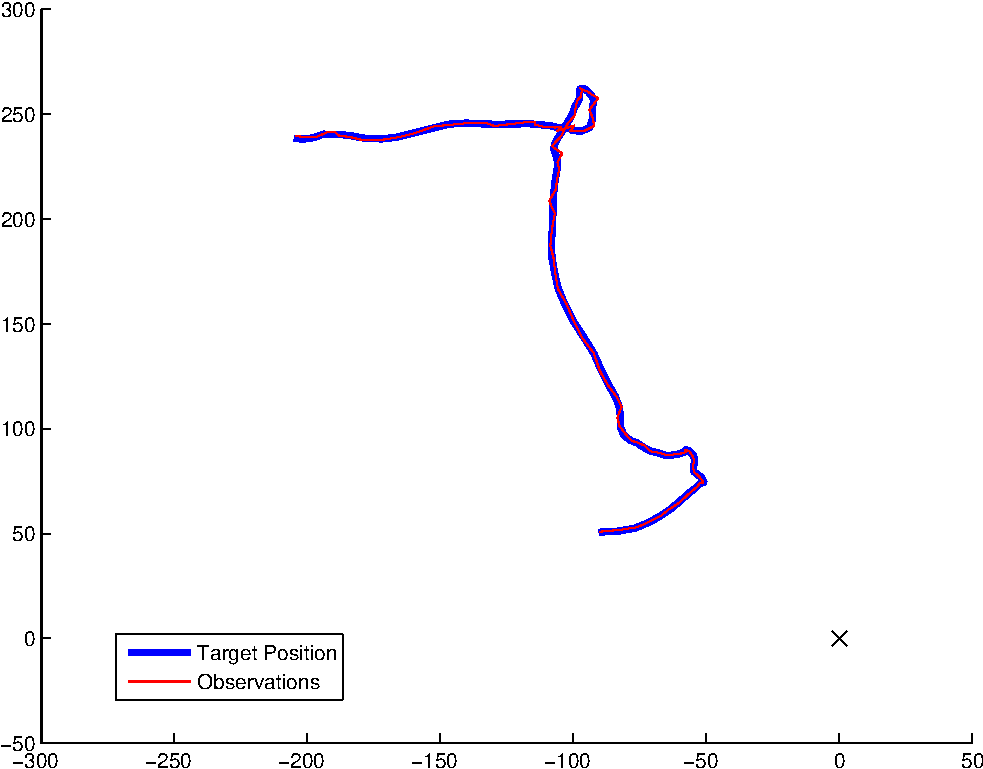
\includegraphics[width=0.45\columnwidth]{case1_trajectory-crop.pdf}%
\label{fig_first_case}}
\hfil
\subfloat[Case 2]{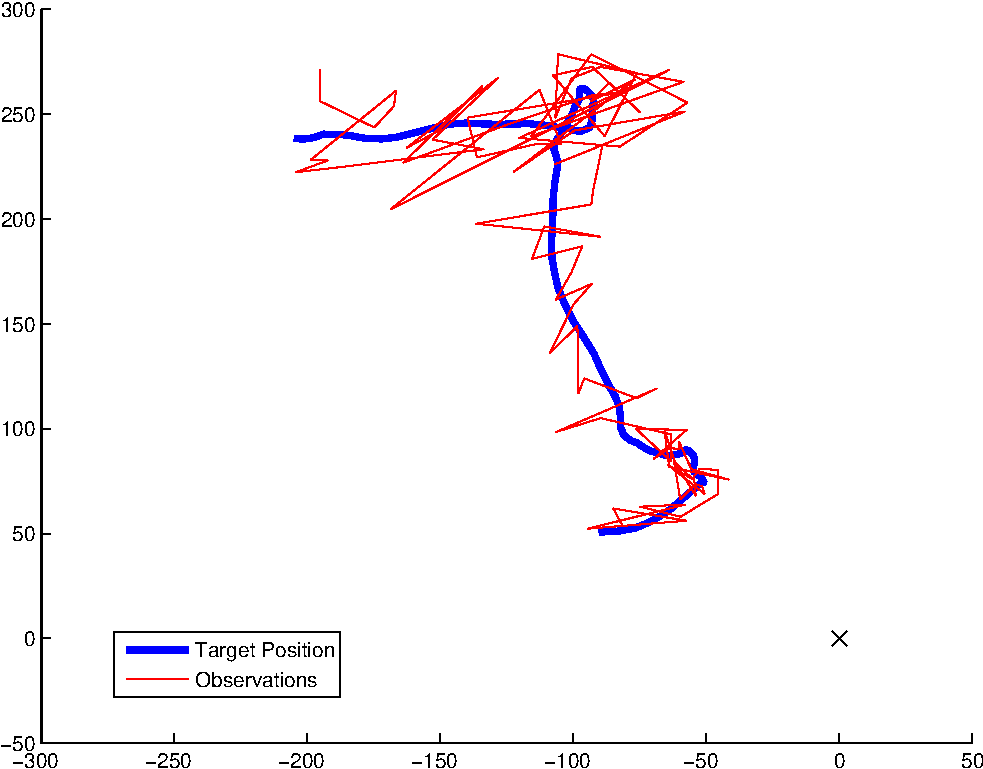
\includegraphics[width=0.45\columnwidth]{case2_trajectory-crop.pdf}%
\label{fig_second_case}}}
\caption{Example trajectory with observations from the two parameter cases.}
\label{fig:example_trajectories}
\end{figure}

Tables~\ref{tab:case1_performance} and~\ref{tab:case2_performance} show the root-mean-square errors (RMSEs) in position and velocity obtained by the different algorithms with the two parameter cases, along with running times (excluding the time for filtering) and the mean number of unique particles at each time instant. The trade-off between speed and error is shown in figures~\ref{fig:case1_rmse_vs_time} and~\ref{fig:case2_rmse_vs_time}.

\begin{table}[!t]%
\renewcommand{\arraystretch}{1.3}
\caption{Smoother performance measures for parameter case 1. All results are averaged over 10 runs, with 500 time steps in each run.}
\label{tab:case1_performance}
\centering
\begin{tabular}{|c||c|c|c|c|}
\hline
Algorithm & \begin{minipage}[c]{1cm} Postion RMSE \end{minipage} & \begin{minipage}[c]{1cm}  Velocity RMSE \end{minipage} & \begin{minipage}[c]{1cm}  Running Time (s) \end{minipage} & \begin{minipage}[c]{1cm}  Unique Particles \end{minipage} \\
\hline
FS 						& 0.578 & 0.968 & 0 & 2.25 \\
DBRS					& 0.475 & 0.762 & 122 & 20.3 \\
\hline
MCMC-BRS (1)	& 0.509 & 0.823 & 3 & 13.7 \\
MCMC-BRS (3)	& 0.493 & 0.790 & 7 & 17.4 \\
MCMC-BRS (10)	& 0.482 & 0.768 & 21 & 19.6 \\
MCMC-BRS (30)	& 0.480 & 0.761 & 62 & 20.2 \\
MCMC-BRS (100)& 0.476 & 0.764 & 202 & 20.4 \\
\hline
MCMC-BSS (1)	& 0.473 & 0.758 & 14 & 44.3 \\
MCMC-BSS (3)	& 0.461 & 0.734 & 29 & 69.7 \\
MCMC-BSS (10)	& 0.451 & 0.720 & 82 & 89.8 \\
MCMC-BSS (30)	& 0.444 & 0.713 & 232 & 96.7 \\
MCMC-BSS (100)& 0.443 & 0.709 & 755 & 98.6 \\
\hline
\end{tabular}
\end{table}

\begin{table}[!t]%
\renewcommand{\arraystretch}{1.3}
\caption{Smoother performance measures for parameter case 2. All results are averaged over 10 runs, with 500 time steps in each run.}
\label{tab:case2_performance}
\centering
\begin{tabular}{|c||c|c|c|c|}
\hline
Algorithm & \begin{minipage}[c]{1cm} Postion RMSE \end{minipage} & \begin{minipage}[c]{1cm}  Velocity RMSE \end{minipage} & \begin{minipage}[c]{1cm}  Running Time (s) \end{minipage} & \begin{minipage}[c]{1cm}  Unique Particles \end{minipage} \\
\hline
FS 						& 6.17 & 2.03 & 0 & 3.96 \\
DBRS					& 5.79 & 1.89 & 63 & 7.34 \\
\hline
MCMC-BRS (1)	& 6.13 & 2.01 & 2 & 4.77 \\
MCMC-BRS (3)	& 6.07 & 1.99 & 4 & 5.29 \\
MCMC-BRS (10)	& 5.94 & 1.94 & 10 & 6.1 \\
MCMC-BRS (30)	& 5.82 & 1.91 & 29 & 6.73 \\
MCMC-BRS (100)& 5.80 & 1.89 & 95 & 7.38 \\
\hline
MCMC-BSS (1)	& 5.90 & 1.91 & 9 & 12.6 \\
MCMC-BSS (3)	& 5.67 & 1.81 & 18 & 22.7 \\
MCMC-BSS (10)	& 5.48 & 1.73 & 50 & 44.1 \\
MCMC-BSS (30)	& 5.43 & 1.69 & 144 & 70.9 \\
MCMC-BSS (100)& 5.34 & 1.68 & 471 & 91.8 \\
\hline
\end{tabular}
\end{table}

\begin{figure}[!t]
\centering
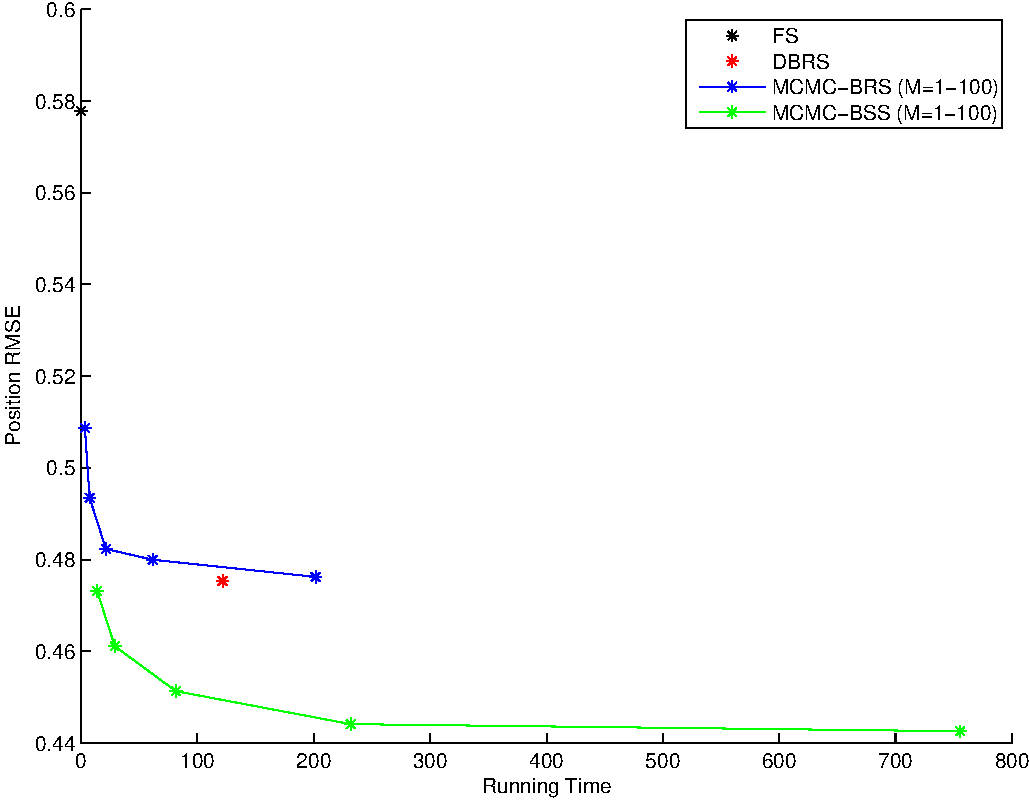
\includegraphics[width=0.8\columnwidth]{case1_smoother_comparison_posRMSE_time-crop.pdf}%
\caption{RMSEs and running times of various smoothing algorithms}%
\label{fig:case1_rmse_vs_time}%
\end{figure}

\begin{figure}[!t]
\centering
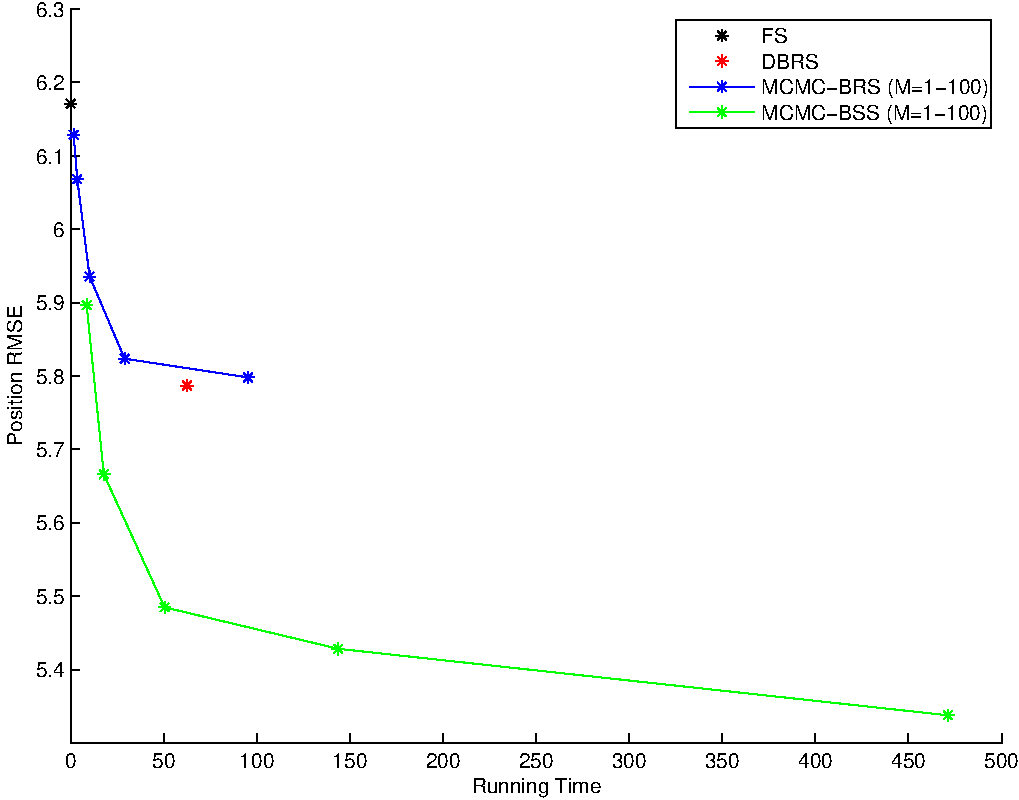
\includegraphics[width=0.8\columnwidth]{case2_smoother_comparison_posRMSE_time-crop.pdf}%
\caption{RMSEs and running times of various smoothing algorithms}%
\label{fig:case2_rmse_vs_time}%
\end{figure}

The MCMC-BRS smoother error approaches that of the DBRS as the number of MCMC steps, $M$, increases. However, for small $M$ the error is only very slightly larger than that of the DBRS but with significantly less running time. For a particular application, it is possible to adjust $M$ to control the trade-off between error and speed.

The MCMC-BSS outperforms all the other smoothers, achieveing a lower RMSE even with $M=1$. As $M$ is increased further, the accuracy increases.



\section{Conclusion} \label{sec:conclusions}
Two new algorithms have been presented for drawing particles from the joint smoothing distribution using MCMC. These MCMC schemes have a degree of flexibility in the choice of chain length, which controls a trade-off between accuracy and running time.

The first algorithm resamples particles from the filtering distributions to produce particles from the smoothing distribution. The error performance of this scheme approaches that of the standard resampling scheme of \cite{Godsill2004} as the chain length increases. However, comparable error performance may be achieved with very short chains with a significant saving in processing time.

The second algorithm samples new values of the state from a continuous proposal density. Although slower than the resampling version for a given length of Markov chain, the error performance is reduced relative to the other smoothers.




%%%% Template bits

% An example of a floating figure using the graphicx package.
% Note that \label must occur AFTER (or within) \caption.
% For figures, \caption should occur after the \includegraphics.
% Note that IEEEtran v1.7 and later has special internal code that
% is designed to preserve the operation of \label within \caption
% even when the captionsoff option is in effect. However, because
% of issues like this, it may be the safest practice to put all your
% \label just after \caption rather than within \caption{}.
%
% Reminder: the "draftcls" or "draftclsnofoot", not "draft", class
% option should be used if it is desired that the figures are to be
% displayed while in draft mode.
%
%\begin{figure}[!t]
%\centering
%\includegraphics[width=2.5in]{myfigure}
% where an .eps filename suffix will be assumed under latex, 
% and a .pdf suffix will be assumed for pdflatex; or what has been declared
% via \DeclareGraphicsExtensions.
%\caption{Simulation Results}
%\label{fig_sim}
%\end{figure}

% Note that IEEE typically puts floats only at the top, even when this
% results in a large percentage of a column being occupied by floats.


% An example of a double column floating figure using two subfigures.
% (The subfig.sty package must be loaded for this to work.)
% The subfigure \label commands are set within each subfloat command, the
% \label for the overall figure must come after \caption.
% \hfil must be used as a separator to get equal spacing.
% The subfigure.sty package works much the same way, except \subfigure is
% used instead of \subfloat.
%
%\begin{figure*}[!t]
%\centerline{\subfloat[Case I]\includegraphics[width=2.5in]{subfigcase1}%
%\label{fig_first_case}}
%\hfil
%\subfloat[Case II]{\includegraphics[width=2.5in]{subfigcase2}%
%\label{fig_second_case}}}
%\caption{Simulation results}
%\label{fig_sim}
%\end{figure*}
%
% Note that often IEEE papers with subfigures do not employ subfigure
% captions (using the optional argument to \subfloat), but instead will
% reference/describe all of them (a), (b), etc., within the main caption.


% An example of a floating table. Note that, for IEEE style tables, the 
% \caption command should come BEFORE the table. Table text will default to
% \footnotesize as IEEE normally uses this smaller font for tables.
% The \label must come after \caption as always.
%
%\begin{table}[!t]
%% increase table row spacing, adjust to taste
%\renewcommand{\arraystretch}{1.3}
% if using array.sty, it might be a good idea to tweak the value of
% \extrarowheight as needed to properly center the text within the cells
%\caption{An Example of a Table}
%\label{table_example}
%\centering
%% Some packages, such as MDW tools, offer better commands for making tables
%% than the plain LaTeX2e tabular which is used here.
%\begin{tabular}{|c||c|}
%\hline
%One & Two\\
%\hline
%Three & Four\\
%\hline
%\end{tabular}
%\end{table}


% Note that IEEE does not put floats in the very first column - or typically
% anywhere on the first page for that matter. Also, in-text middle ("here")
% positioning is not used. Most IEEE journals use top floats exclusively.
% Note that, LaTeX2e, unlike IEEE journals, places footnotes above bottom
% floats. This can be corrected via the \fnbelowfloat command of the
% stfloats package.








% if have a single appendix:
%\appendix[Proof of the Zonklar Equations]
% or
%\appendix  % for no appendix heading
% do not use \section anymore after \appendix, only \section*
% is possibly needed

% use appendices with more than one appendix
% then use \section to start each appendix
% you must declare a \section before using any
% \subsection or using \label (\appendices by itself
% starts a section numbered zero.)
%


%\appendices
%\section{Appendix Title}
%Appendix one text goes here.

% you can choose not to have a title for an appendix
% if you want by leaving the argument blank
%\section{}
%Appendix two text goes here.


% use section* for acknowledgement
%\section*{Acknowledgment}


%The authors would like to thank...


% Can use something like this to put references on a page
% by themselves when using endfloat and the captionsoff option.
\ifCLASSOPTIONcaptionsoff
  \newpage
\fi



% trigger a \newpage just before the given reference
% number - used to balance the columns on the last page
% adjust value as needed - may need to be readjusted if
% the document is modified later
%\IEEEtriggeratref{8}
% The "triggered" command can be changed if desired:
%\IEEEtriggercmd{\enlargethispage{-5in}}

% references section

% can use a bibliography generated by BibTeX as a .bbl file
% BibTeX documentation can be easily obtained at:
% http://www.ctan.org/tex-archive/biblio/bibtex/contrib/doc/
% The IEEEtran BibTeX style support page is at:
% http://www.michaelshell.org/tex/ieeetran/bibtex/
\bibliographystyle{IEEEtran}
\bibliography{D:/pb404/Dropbox/PhD/OTbib}

% biography section
% 
% If you have an EPS/PDF photo (graphicx package needed) extra braces are
% needed around the contents of the optional argument to biography to prevent
% the LaTeX parser from getting confused when it sees the complicated
% \includegraphics command within an optional argument. (You could create
% your own custom macro containing the \includegraphics command to make things
% simpler here.)
%\begin{biography}[{\includegraphics[width=1in,height=1.25in,clip,keepaspectratio]{mshell}}]{Michael Shell}
% or if you just want to reserve a space for a photo:

\begin{IEEEbiographynophoto}{Pete Bunch}
Biography text here.
\end{IEEEbiographynophoto}

% if you will not have a photo at all:
\begin{IEEEbiographynophoto}{Simon Godsill}
Biography text here.
\end{IEEEbiographynophoto}

% insert where needed to balance the two columns on the last page with
% biographies
%\newpage

% You can push biographies down or up by placing
% a \vfill before or after them. The appropriate
% use of \vfill depends on what kind of text is
% on the last page and whether or not the columns
% are being equalized.

%\vfill

% Can be used to pull up biographies so that the bottom of the last one
% is flush with the other column.
%\enlargethispage{-5in}



% that's all folks
\end{document}


